\documentclass[thesis.tex]{subfiles}

\begin{document}

\chapter{Evaluation}\label{chap:eva}
This chapter will evaluate the proposed algorithms both from a performance and a quality perspective.
In the last section we try to compare our technique to others.
However, as we were not able to implement comparable implementations within the bounds of this project, we can only provide comparisons on an abstract level.

\section{Test Setup \& Scenes} \label{sec:eva:setup}
All tests were rendered using a Nvidia GTX670 desktop graphics card.
The test machine contains a Intel i7-3770 CPU and uses Windows 8 64bit as OS.

\begin{figure}
\centering
\begin{subfigure}[b]{0.8\textwidth}
\centering
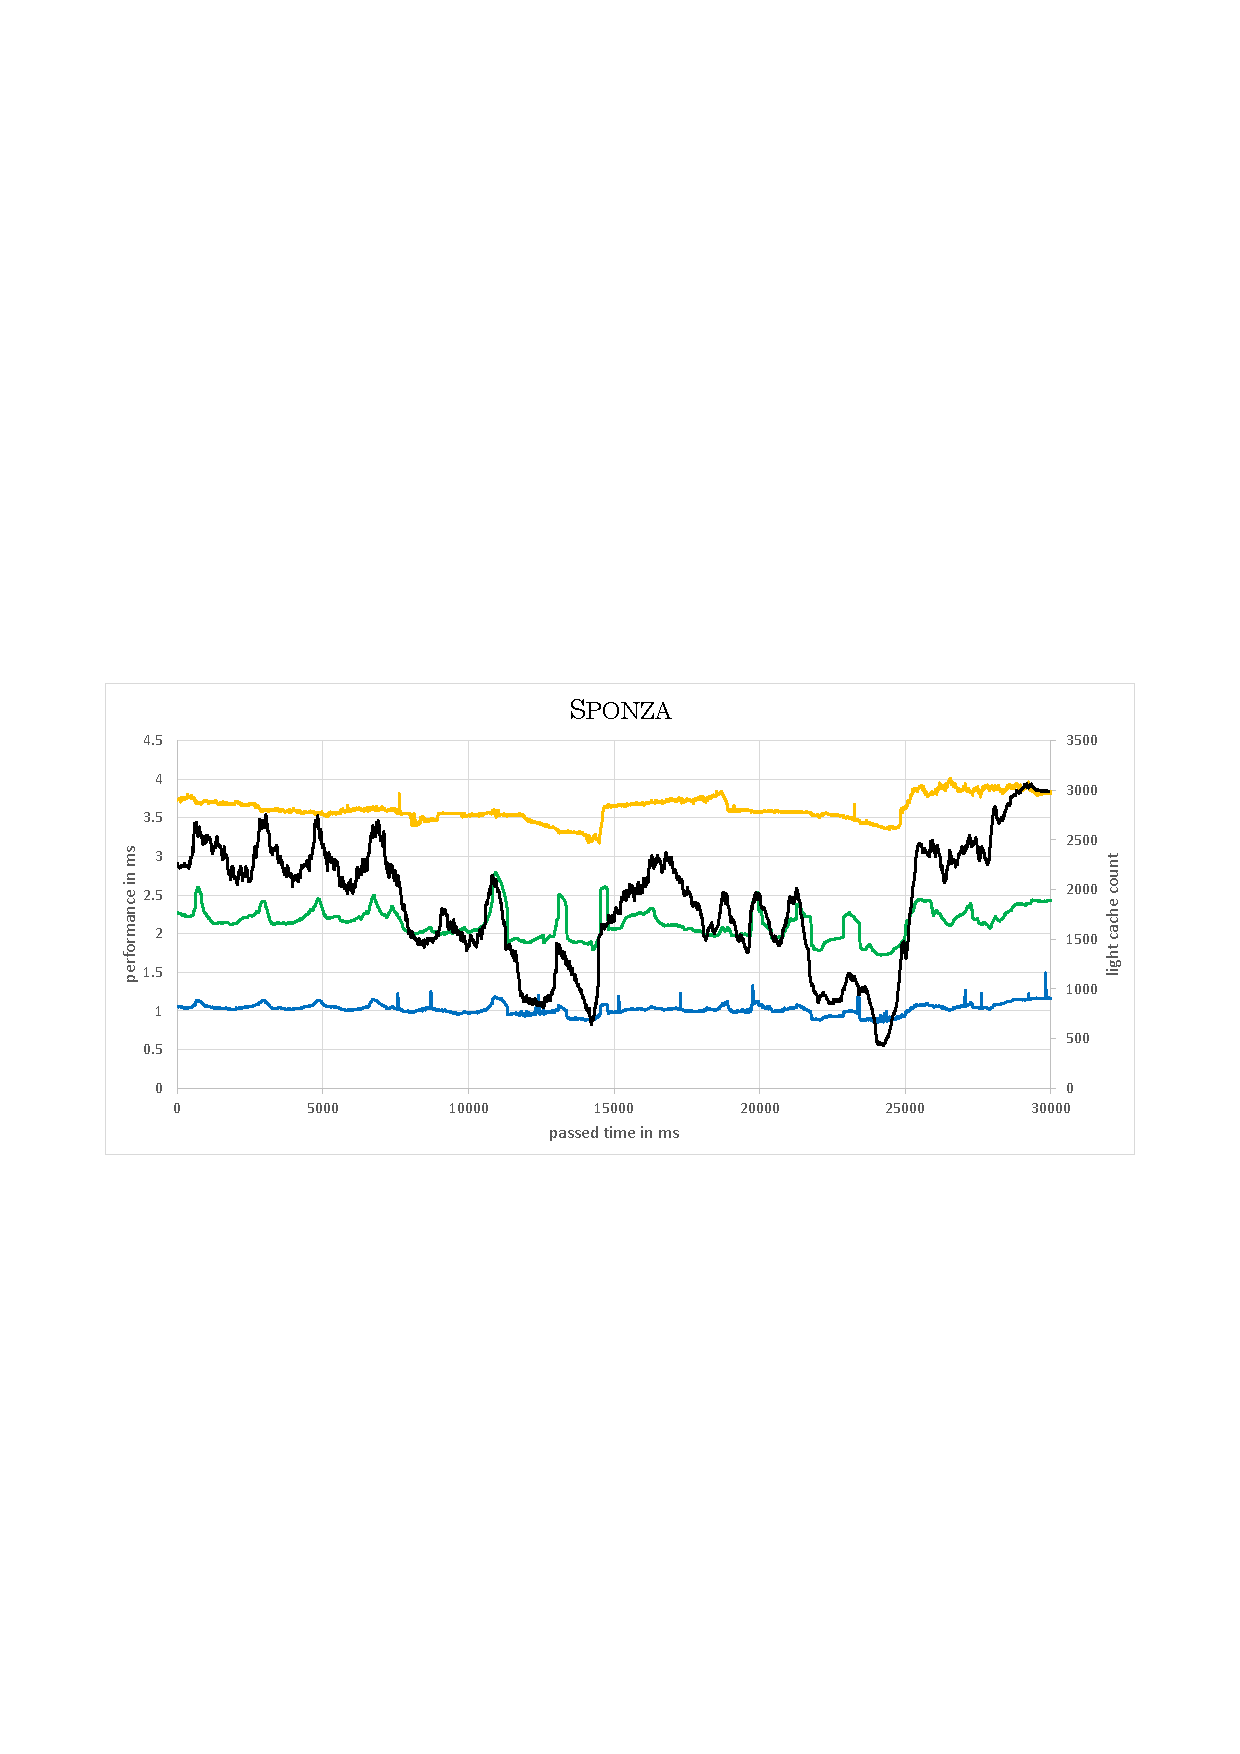
\includegraphics[width=\textwidth]{eva/scenes/sponza}
\caption{\dataset{Sponza}}
\end{subfigure}
\\
\begin{subfigure}[b]{0.8\textwidth}
\centering
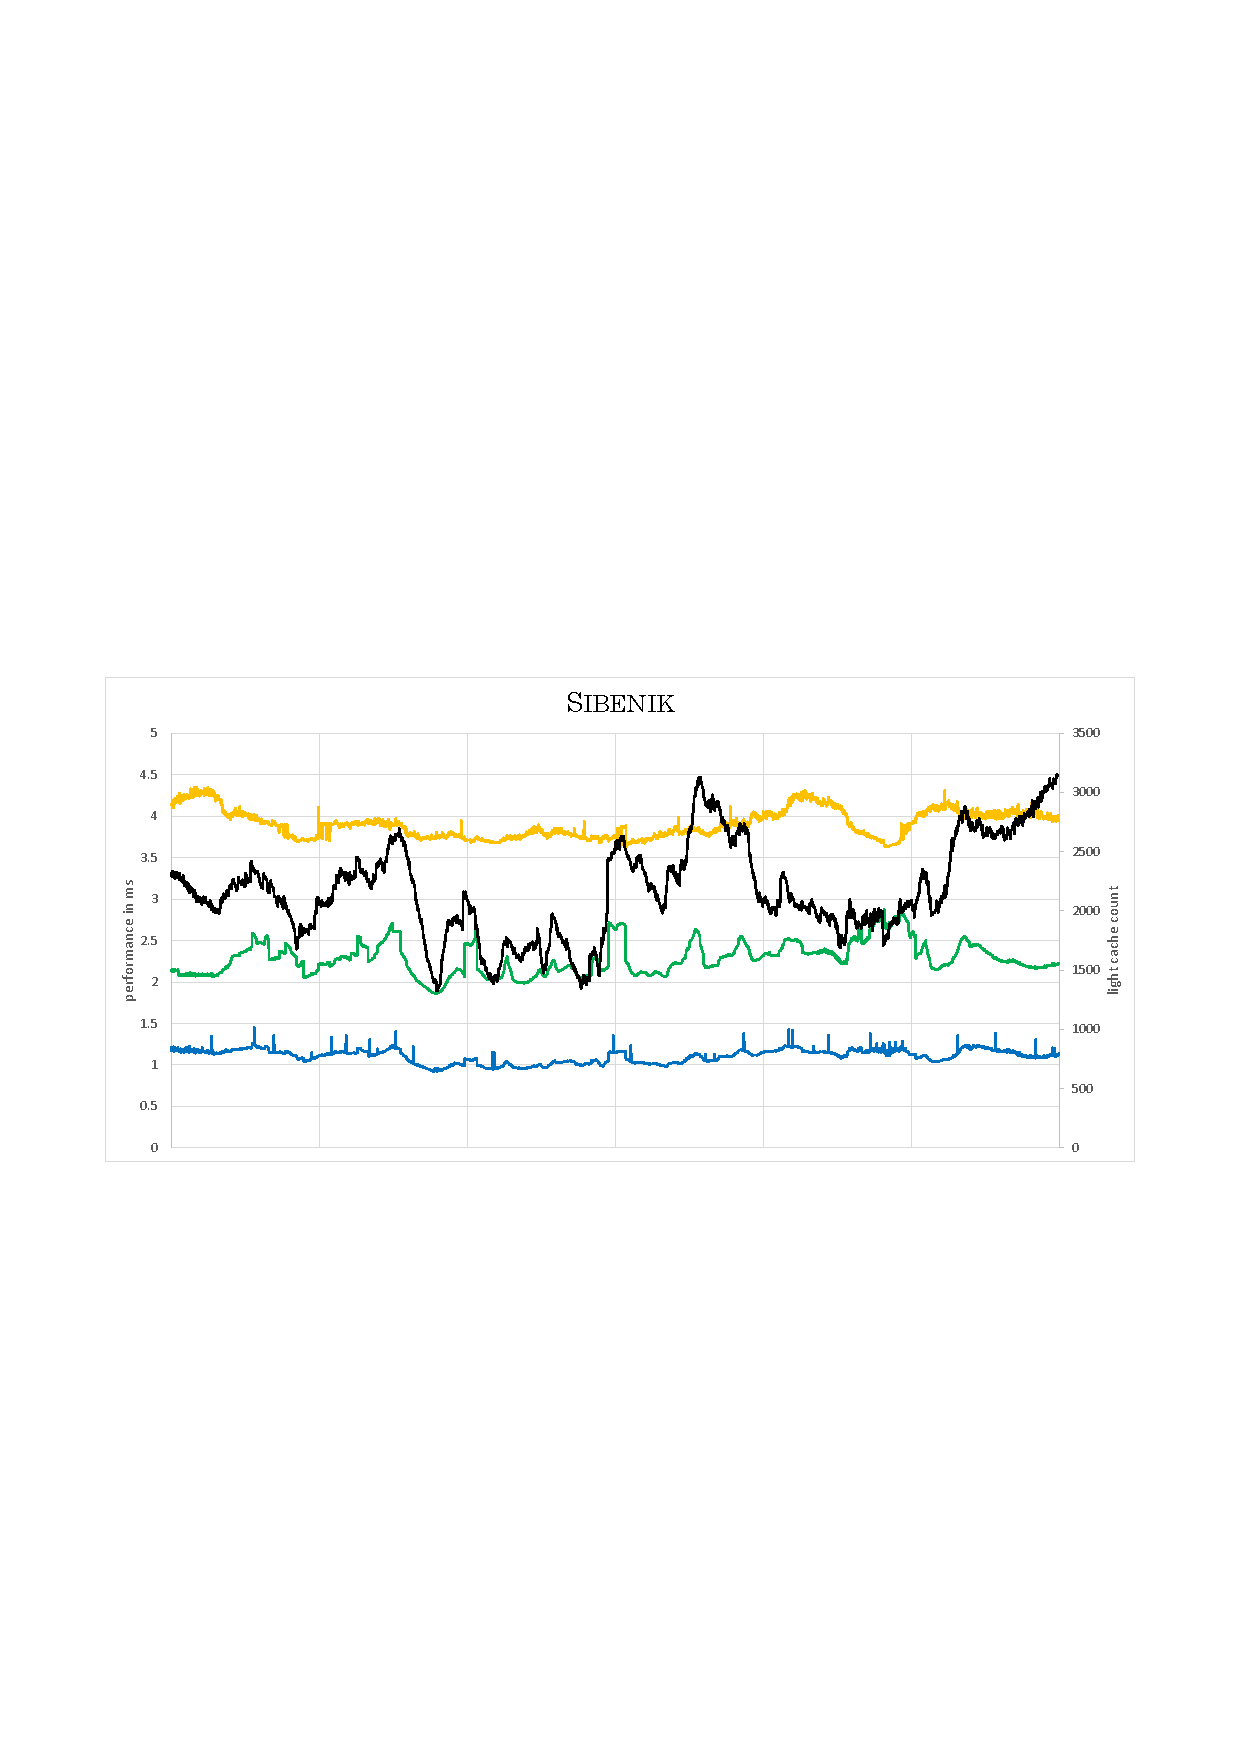
\includegraphics[width=\textwidth]{eva/scenes/sibenik}
\caption{\dataset{Sibenik}}
\end{subfigure}
\\
\begin{subfigure}[b]{0.8\textwidth}
\centering
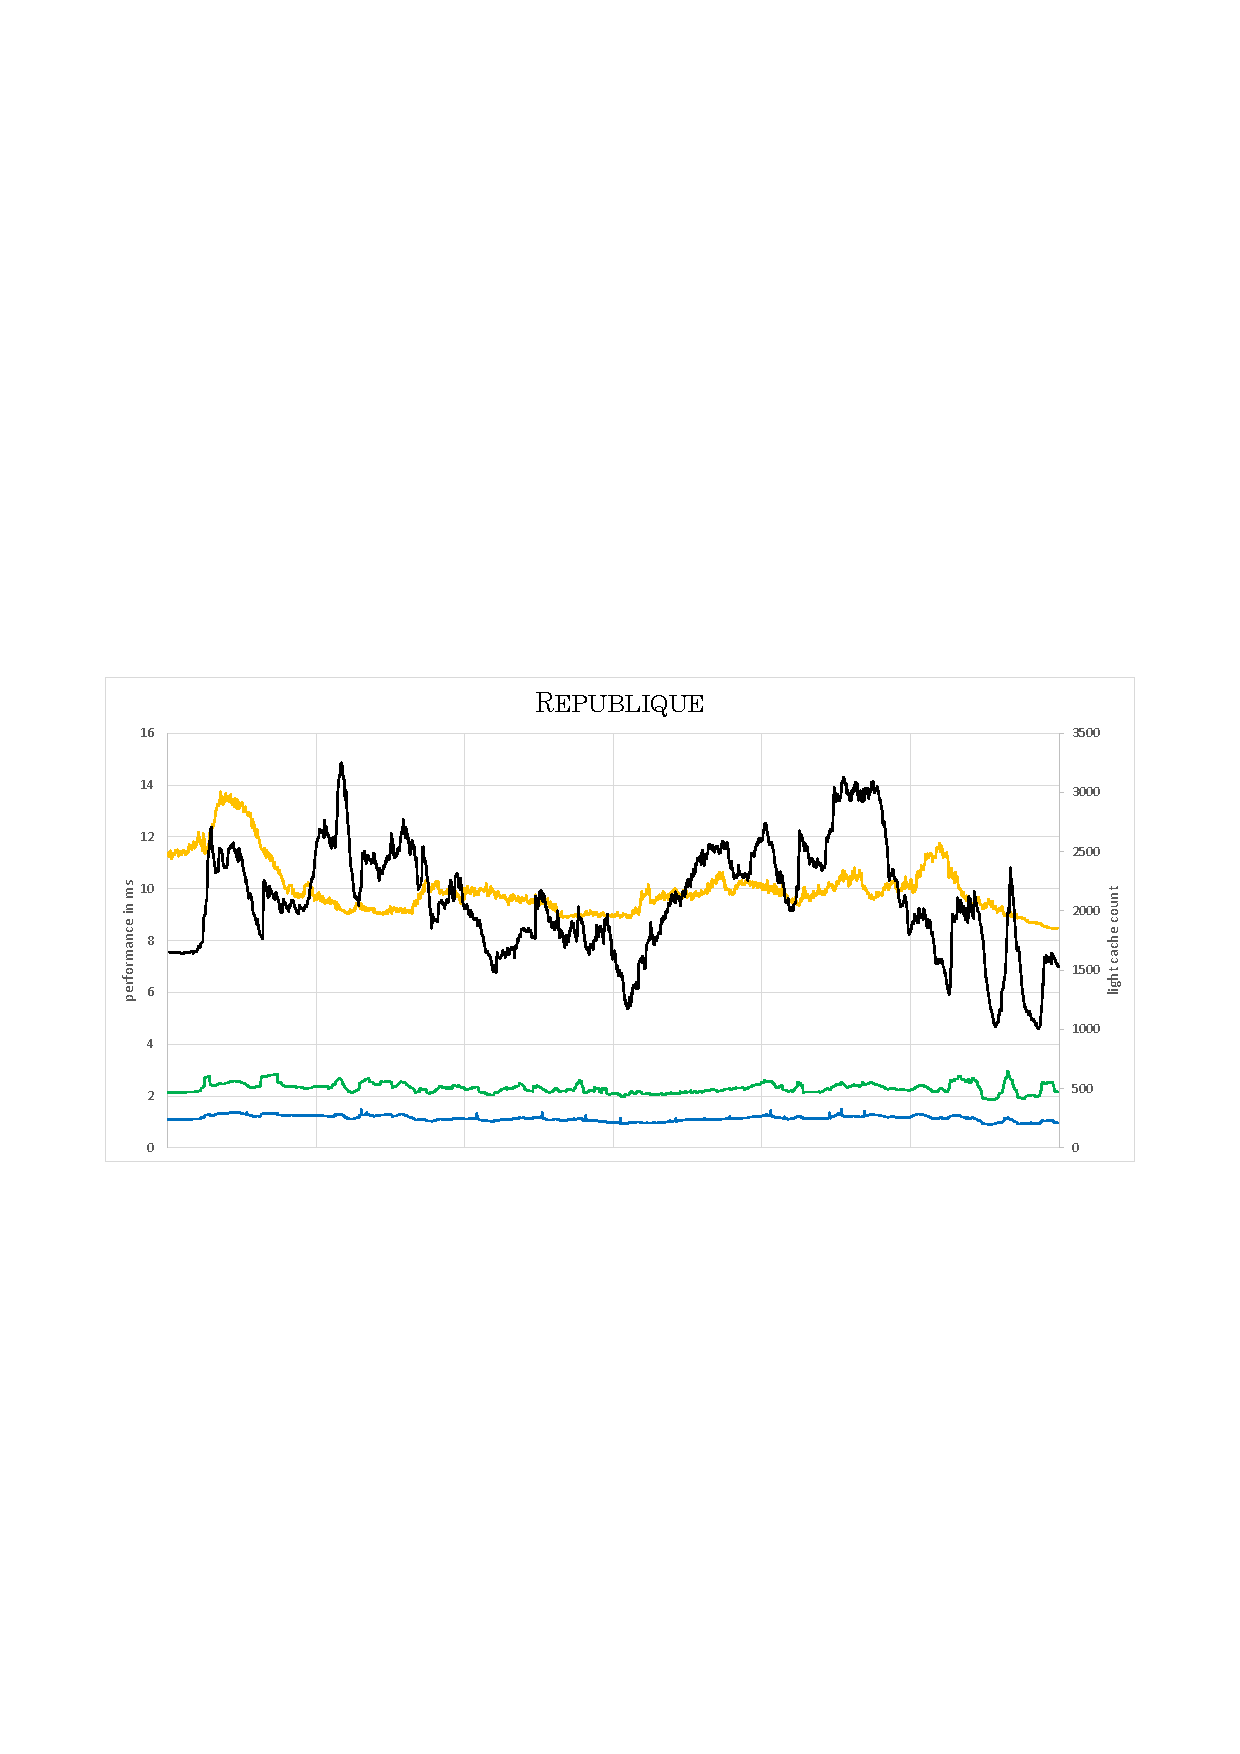
\includegraphics[width=\textwidth]{eva/scenes/republique}
\caption{\dataset{Republique}}
\end{subfigure}
\caption{Overview over our three main test scenes.}
\label{fig:testscenes}
\end{figure}
\autoref{fig:testscenes} gives an overview over the main test scenes used in this chapter (and throughout the thesis).
We use McGuire's \cite{bib:McGuire2011Data} version of the well known Crytek \dataset{Sponza} scene which was modeled by Frank Meinl.
For a better fit into our physically based pipeline we used the freely provided texture set  by Alexandre Pestana \cite{bib:sponzapbr}.
\\
The \dataset{Sibenik} cathedral scene is as well from McGuire's database \cite{bib:McGuire2011Data}.
To fill the empty space, we added a dinosaur skeleton from the "Natural History Museeum" modelled by Alvara Luna Bautista and Joel Anderson (available at \url{http://www.3drender.com/challenges/}).
\\
The \dataset{Republique} scene was extracted from a unity tech demo for the game "République Remastered" by Camouflaj.
The entire demo is freely available on the unity assetstore \cite{bib:republique}.

\section{Parameter Overview}
How our approach performs depends on several parameters.
To make this chapter more readable and make comparisons easier, we use a standard configuration on all parameters that are not mentioned explicitly.
Those defaults are annotated in brackets in this list:
\begin{easylist}
\ListProperties(Hide=100, Hang=true, Progressive=4ex, Space=0.0ex, Space3=-0.5ex, Space*=-0.5ex, Style*=$\bullet\,$,
Style2*=\textbf{--} ,Style3*=$\circ$ ,Style4*=\tiny$\blacksquare$ )
# general
## screen resolution ($1920\times1080$)
## number of lights (a single spot light)
## reflective shadow map resolution (rendering $1024^2$, indirect light $64^2$)
## number of SH bands for diffuse lighting (2 bands)
## number of active caches
### cache address volume resolution ($32^3$)
### cascading settings (4 cascades, last cascade covers always entire scene)
### camera
# shadowing
## shadow lod (2)
## voxel resolution ($128^3$)
# specular
## specular environment map resolution ($16^2$)
## direct write or cached write (direct write)
\end{easylist}
This chapter tries to give insights on their effects.
We limit our observation to meaningful ranges and do not experiment with arbitrary combinations.

 \todo{write why voxel res is bad}

\section{Performance}
In this section the performance and scalability of our approach is examined.
We measure primarily frame times in milliseconds.
To be able to evaluate how specific parts of our algorithm perform, we use OpenGLs timer query functionality to check how long a series of calls take to finish on the GPU (\texttt{GL\_TIME\_ELAPSED}).
The sum of timings from multiple commands may exceed the time a frame takes, since the GPU might work on multiple commands at a time.
However, in our tests this overlap seems to play a minor role since most tasks are either very computational intense or are depending on each other which prohibits parallel command execution.

\subsection{General Breakdown}
First we want to provide a general overview over how long the different steps of our rendering pipeline usually take.
For this we measure all timings along 30 seconds camera flights through our test scenes using the default settings mentioned in \autoref{sec:eva:setup}.
\begin{figure}
\centering
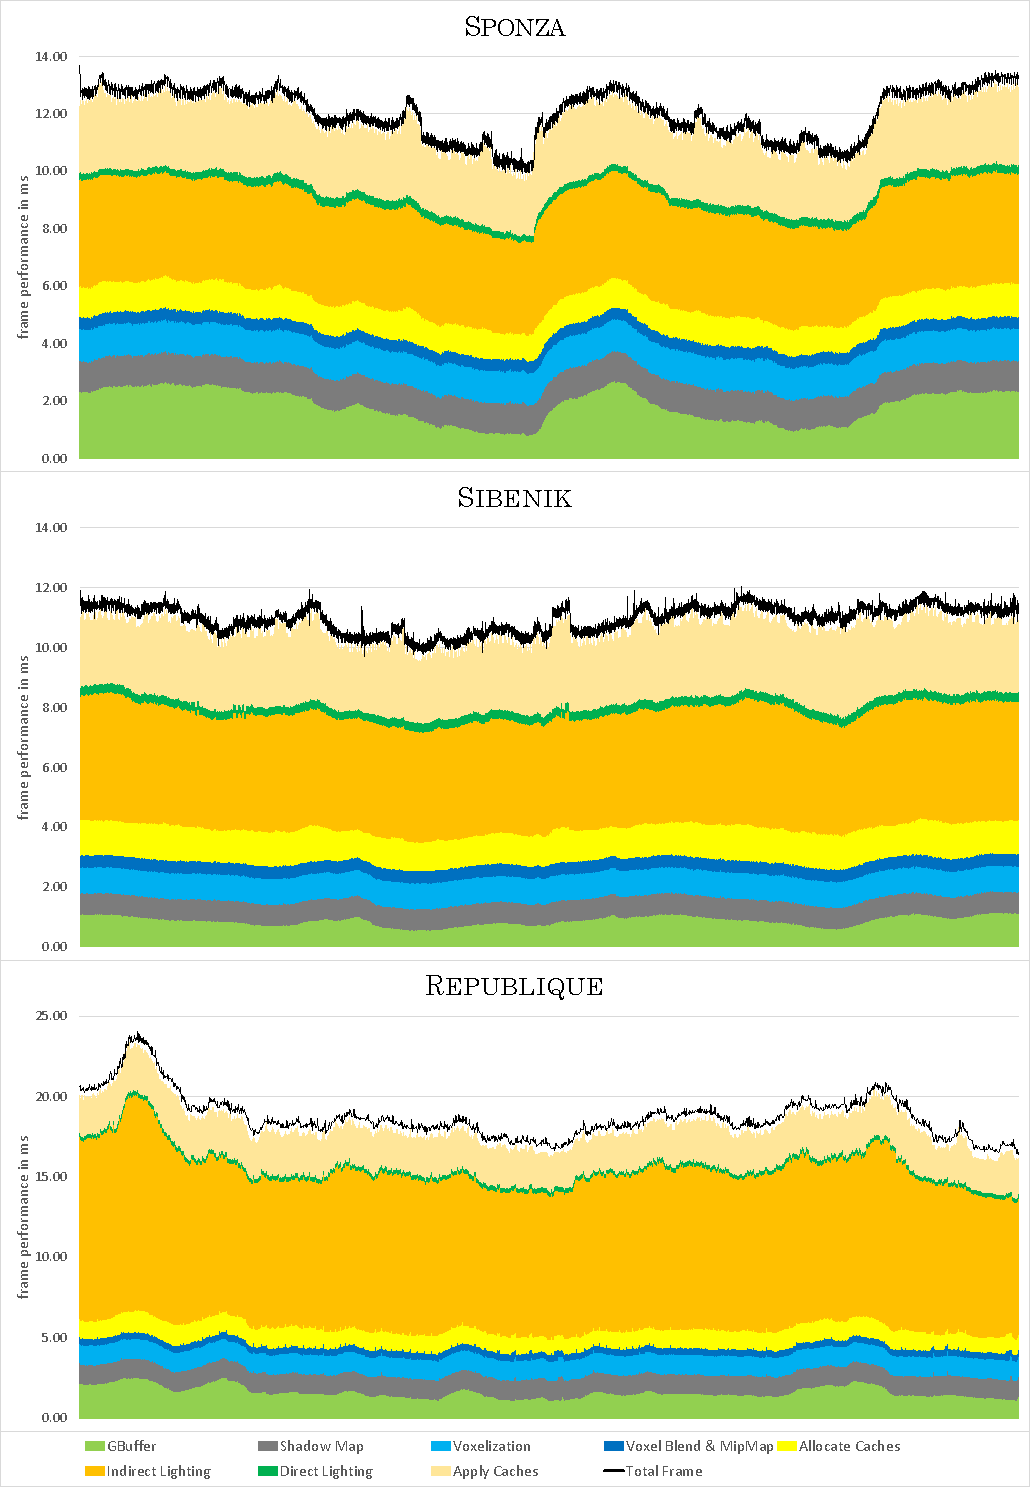
\includegraphics[width=\textwidth]{eva/breakdown/specoff.pdf}
\caption{Breakdown of frame timings with a moving camera over time (30s) for indirect diffuse lighting with shadowing.}
\label{fig:frameratebreakdown:specoff}
\end{figure}

\begin{figure}
\centering
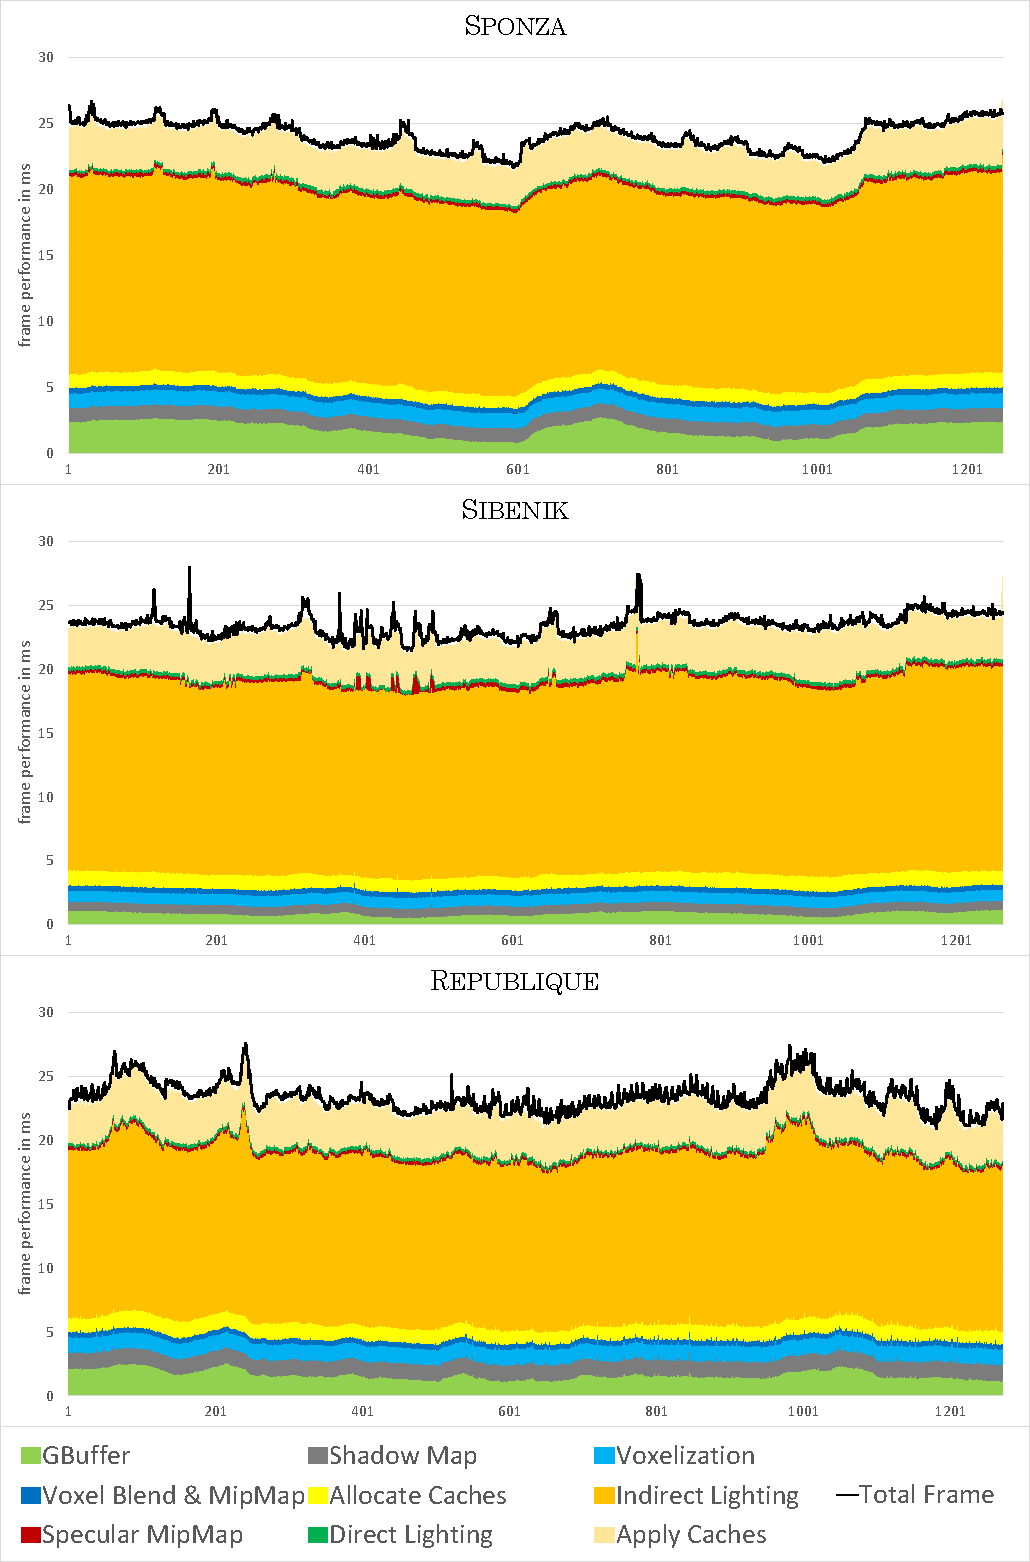
\includegraphics[width=\textwidth]{eva/breakdown/specon.pdf}
\caption{Breakdown of frame timings with a moving camera over time (30s) for indirect diffuse \& \emph{specular} lighting with shadowing.}
\label{fig:frameratebreakdown:specon}
\end{figure}

\subsection{Cache Count}
Examine effect of different cachte counts, cascading, CAV, etc.

\subsection{Resolution Dependence}
Examine effect of resolution on prepare and apply passes.

\subsection{Indirect Shadow}


\subsection{Indirect Specular}

\newpage

\section{Quality}
% phenomelogical: "Quality of light, shadow, etc." - which parameters need to be tweaked

\subsection{Sources of Error and Groundtruth Comparision}
Shadow heuristic check! (try to use only one)

\subsection{Artifacts}
regular placement of caches, jaggies,
shadow jaggies,
/interpolation issues

shadow flickering?

\subsection{Temporal Coherency}


\section{Memory Consumption}

\section{Comparison to other Techniques} \label{sec:eva:comparisiontoother}

comparison table, similar to the one in radiance hints?

\subsection{Comparison to LightSkin}

\subfilebib % Makes bibliography available when compiling as subfile
\end{document}